\input{../../headers/tdheaders.tex}

\section{Pompe Milroyal}

Une pompe est un dispositif permettant d'aspirer et de refouler un fluide. 
\subsection{Pompe à piston}

\begin{figure}[htbp]
\begin{minipage}[c]{.4\linewidth}
\begin{center}
\includegraphics[width=\linewidth]{img/pompe_piston}
\caption{Pompe à piston Milroyal}
\label{fig:image1}
\end{center}
\end{minipage}
\hfill
\begin{minipage}[c]{.55\linewidth}
 
 Ce type de pompe utilise un piston coulissant de manière étanche dans un cylindre pour repousser un fluide, admis précédemment dans le cylindre par l'intermédiaire d'un clapet, d'une soupape ou d'une lumière, grâce à l'aspiration provoquée par le recul du piston.

Les performances sont élevées :

\begin{itemize}
 \item Pression de plusieurs milliers de bar, notamment pour le découpage jet d'eau
 \item Débit jusqu'à 500 litres/min
 \item Rendement > 0,951
\end{itemize}

\end{minipage}
\end{figure}

Il existe différents montages mécaniques dont :
\begin{itemize}
 \item Pompe à pistons axiaux \ref{fig:image1}.

Les pistons sont situés parallèlement à l'axe de transmission. 

 \item Pompe à pistons radiaux

Les patins des pistons glissent sur un excentrique ou sur une came dont le nombre de lobes est différent (de un) au nombre de pistons. Les pistons sont munis de clapets d'aspiration et de refoulement. Souvent, pour des raisons de régularité de flux, le nombre de pistons est impair (somme de sinusoïdes régulièrement déphasées).

\item Pompe à vilebrequin

Dans le cas de l'utilisation d'un fluide non lubrifiant comme de l'eau, avec de gros débits et / ou de fortes pressions, un vilebrequin entraîne un ensemble de pistons en ligne. Ces pompes particulièrement chères sont rarement utilisées.
\end{itemize}

\begin{figure}[htbp]
\begin{minipage}[c]{.55\linewidth}
Dans, les pompes hydraulique à pistons axiaux, figure \ref{fig:image2} (aussi appelées pompes oléohydraulique), les pistons sont situés parallèlement ou inclinés part rapport à l'axe d'entraînement. Le c\oe ur de la pompe est constitué d'un barillet, de glaces de distribution et de pistons.
\end{minipage}
\hfill
\begin{minipage}[c]{.4\linewidth}
\begin{center}
\includegraphics[width=\linewidth]{img/pompe_axiaux.jpg}
\caption{Pompe à piston axiaux}
\label{fig:image2}
\end{center}
\end{minipage}
\end{figure}

Elle pénètre tous les secteurs : agriculture, industrie, sidérurgie, aéronautique, travaux publics, etc.

\begin{itemize}
 \item Excellent rapport poids / puissance
 \item Régime de rotation élevée, grâce à la faible inertie des masses tournantes
 \item Cylindrée élevée et le régime rapide permet de très grosse puissance
 \item Pression plus de 6000 psi (420 bars)
 \item Le bon rapport qualité prix en fait une des pompes les plus courantes après les pompes à engrenages
 \item Distribution par glace sans clapets, ce qui les rend auto amorçante
 \item La technologie est souvent réversible en moteur
 \item Cylindrée fixe ou variable
 \item Rendements mécaniques et volumétriques corrects
\end{itemize}

\paragraph{Question 1:}
Sur le dessin de définition, colorier les classes d'équivalence du mécanisme étudié.

\paragraph{Question 2:}

Proposer un graphe des liaisons du mécanisme en ajoutant les noms, axes et mobilités des liaisons.

\paragraph{Question 3:}

Déterminer la course du piston de cette pompe, ainsi que la cylindrée et enfin le débit en supposant une vitesse de rotation du moteur de $1000 tr.min^{-1}$.

\textit{Un réglage est possible sur cette pompe}

\paragraph{Question 4:}

Décrire le fonctionnement de ce réglage ainsi que la grandeur sur laquelle il intervient (débit, pression,...).

\newpage

\includepdf[angle=90,offset=6mm -7mm]{img/Milroyal_2.pdf}

\includepdf[angle=90,offset=7mm -7mm]{img/Milroyal_3.pdf}

\newpage

\section{Chaise de dentiste}

\subsection{Mise en situation}

\begin{figure}[htbp]
\begin{minipage}[c]{.4\linewidth}
\begin{center}
\includegraphics[width=\linewidth]{img/cabinet.jpg}
\caption{Fauteuil dans un cabinet}
\label{fig:image3}
\end{center}
\end{minipage}
\hfill
\begin{minipage}[c]{.55\linewidth}
La chirurgie dentaire et ses spécificités opératoires nécessitent l'installation du patient dans une position couchée particulière (voir illustration ci-dessous). La société AIREL a donc développé un fauteuil d'opération ergonomique, véritable automate comportant toutes les commandes et les fonctions dont le praticien doit disposer, quelle que soit sa spécialité et ses contraintes opératoires.
\end{minipage}
\end{figure}

\subsection{Présentation du système}

\begin{figure}[htbp]
\begin{minipage}[c]{.5\linewidth}
Le système de levée du fauteuil, qui va être l'objet de notre étude, est composé d'un vérin ainsi que d'un système pantographe.

Il permet de piloter la montée et la descente du fauteuil afin de placer le patient à une hauteur adéquate afin que le médecin pratique son intervention dans les meilleures conditions possibles.
\end{minipage}
\hfill
\begin{minipage}[c]{.45\linewidth}
\begin{center}
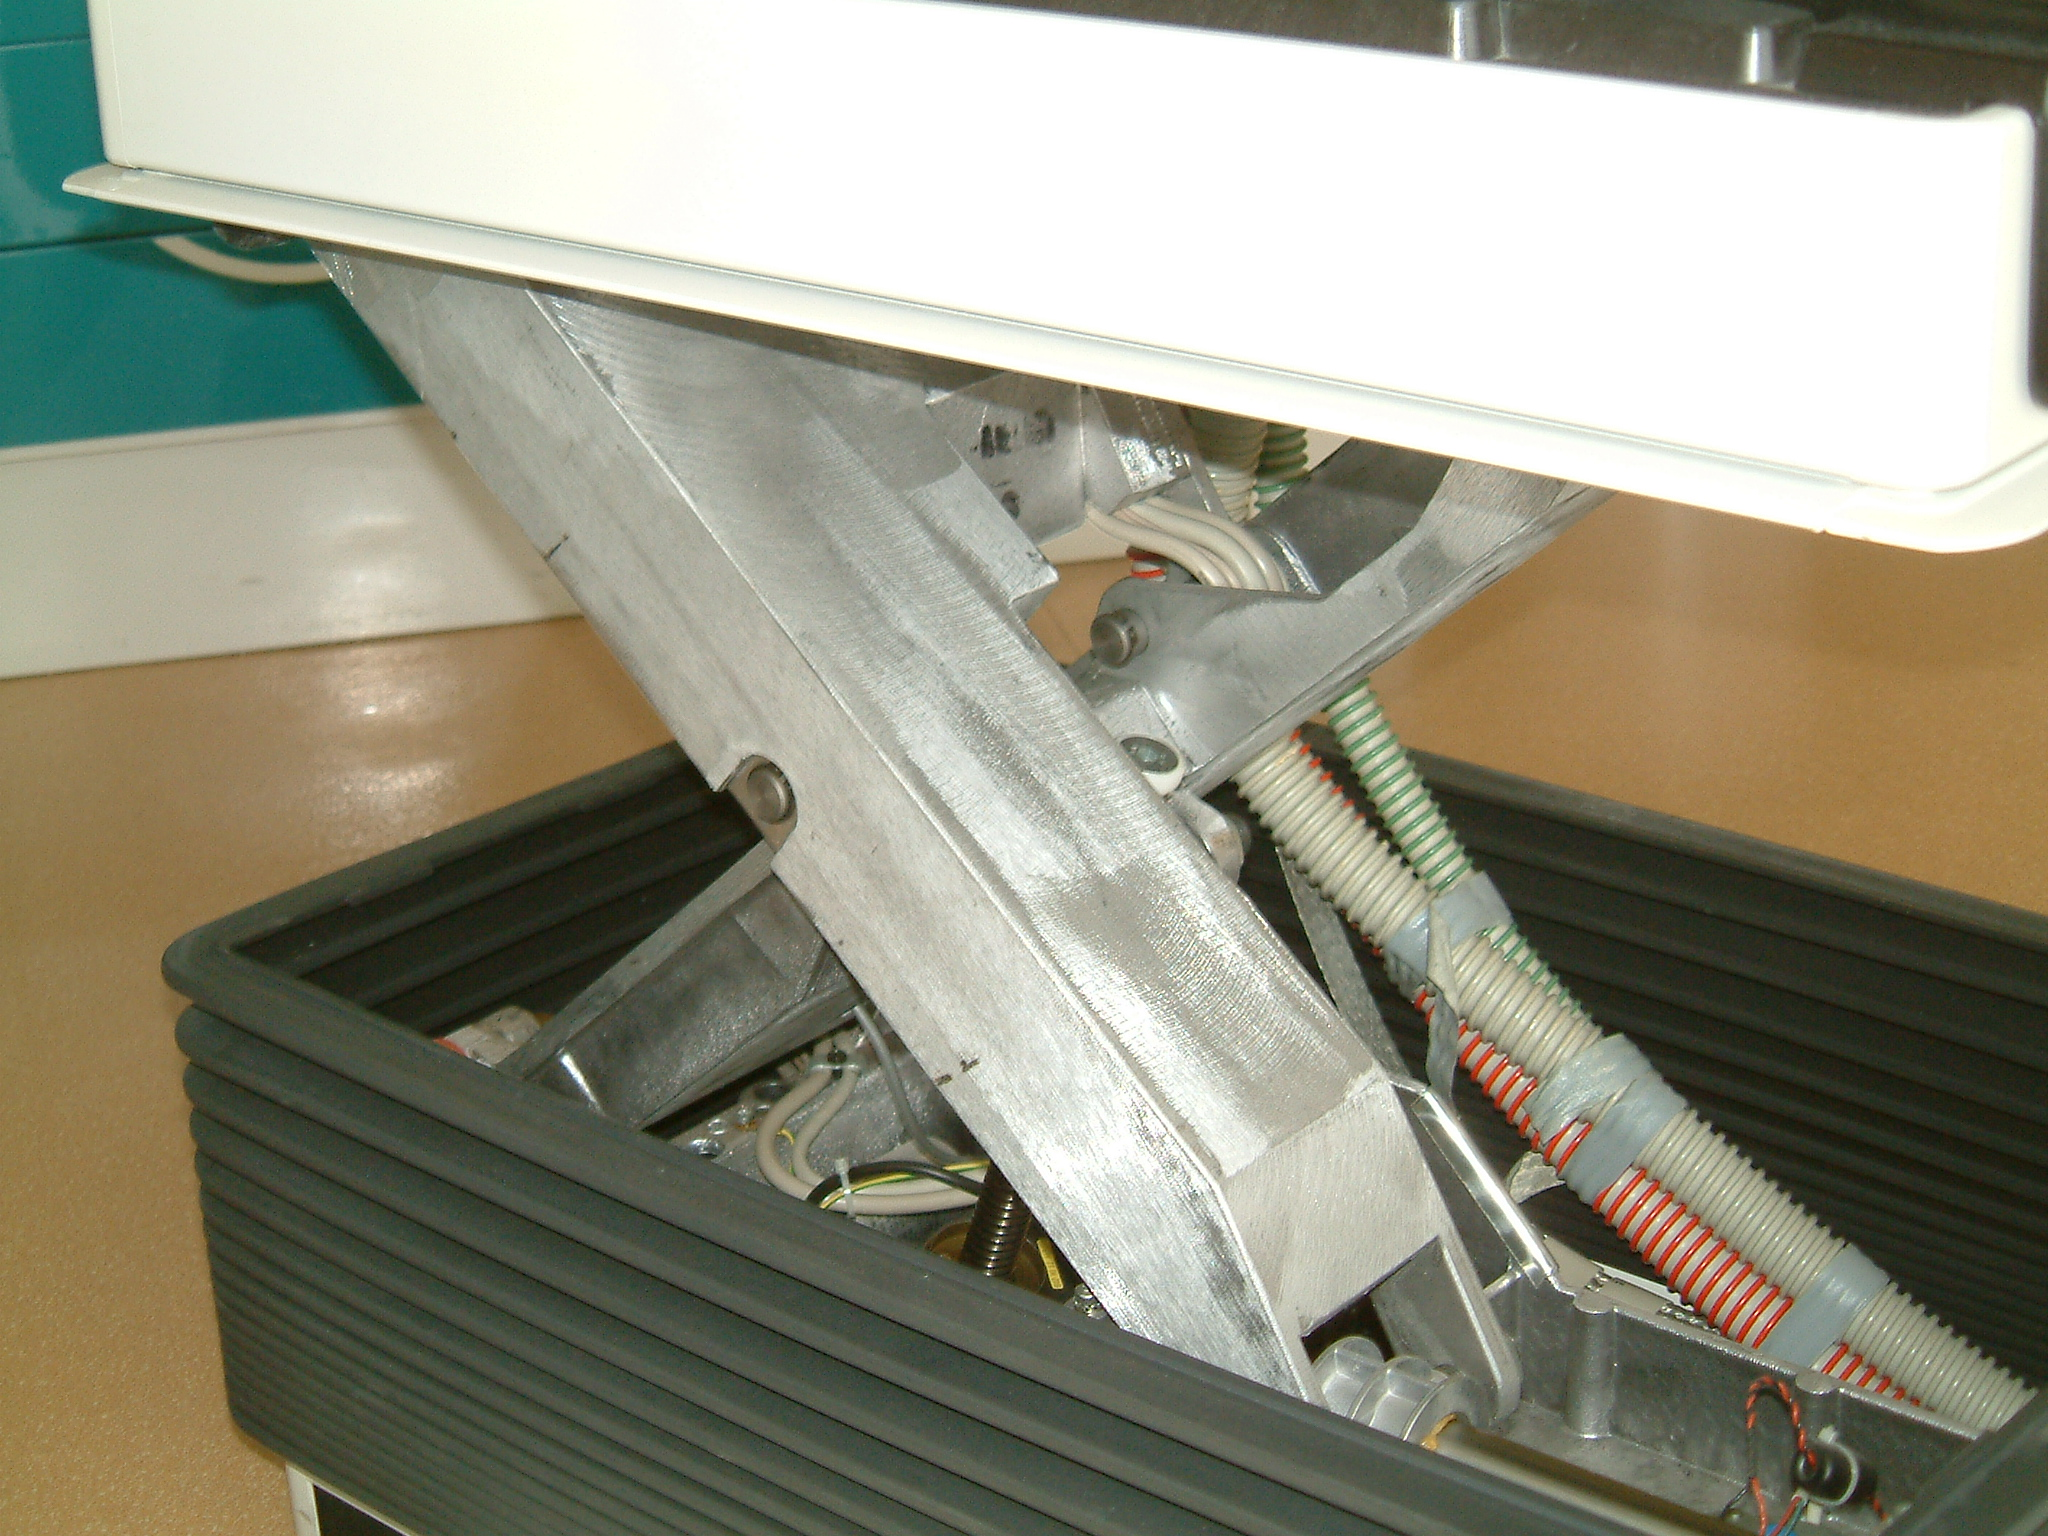
\includegraphics[width=\linewidth]{img/detail_chaise.png}
\caption{Système de levée}
\label{fig:image4}
\end{center}
\end{minipage}
\end{figure}

Deux pièces ont été extraites du mécanisme: le bras 4 et la pièce 9.

\paragraph{Question 1:}

Représenter le bras 4 sur trois vues à choisir le plus judicieusement possible.

\paragraph{Question 2:}

Représenter la pièce 9 sur trois vues à choisir le plus judicieusement possible.

Des vues de ces pièces sont donnée sur les figures \ref{fig:image5}, \ref{fig:image6} et \ref{fig:image7}.

\begin{figure}[htbp]
\begin{minipage}[c]{.5\linewidth}
\begin{center}
\includegraphics[width=\linewidth]{img/face.png}
\caption{Vue du bras 4 intégré au système}
\label{fig:image5}
\end{center}
\end{minipage}
\hfill
\begin{minipage}[c]{.45\linewidth}
\begin{center}
\includegraphics[width=0.9\linewidth]{img/Bras}
\caption{Vue du bras 4}
\label{fig:image55}
\end{center}
\end{minipage}
\end{figure}

\begin{figure}[htbp]
\begin{minipage}[c]{.4\linewidth}
\begin{center}
\includegraphics[width=0.9\linewidth]{img/palier1.png}
\caption{Vue de la pièce 9}
\label{fig:image6}
\end{center}
\end{minipage}
\hfill
\begin{minipage}[c]{.4\linewidth}
\begin{center}
\includegraphics[width=0.9\linewidth]{img/palier2.png}
\caption{Vue de la pièce 9}
\label{fig:image7}
\end{center}
\end{minipage}
\end{figure}

\ifdef{\public}{\end{document}}{}

\newpage

\pagestyle{correction}

\section{Correction}

\subsection{Pompe Milroyal}

\paragraph{Question 1:}

\begin{center}
 \includegraphics[width=0.9\linewidth]{img/Milroyal_mobilites}
\end{center}

\paragraph{Question 2:}

\begin{center}
 \includegraphics[width=0.65\linewidth]{img/Liaisons}
\end{center}

\newpage

\paragraph{Question 3:}

\begin{center}
 \includegraphics[width=0.8\linewidth]{img/Milroyal_course}
\end{center}

La course est alors de $22mm$.

Le diamètre est de $22mm$, la section est donc de $380mm^2$, ce qui génère un volume de $8362mm^3$.

Le débit est donc de $8362x1000mm^3.min^(-1)$, soit $8.3L.min^(-1)$.

\newpage

\paragraph{Question 4:}

\begin{center}
 \includegraphics[width=0.9\linewidth]{img/Milroyal_4}\\
 \includegraphics[width=0.9\linewidth]{img/Milroyal_5}
\end{center}

\subsection{Chaise de dentiste}

\includepdf[offset=7mm -7mm,width=1.15\linewidth]{img/Palier_guide_corrige.pdf}

\includepdf[offset=7mm -7mm,width=1.15\linewidth]{img/Palier_guide_pointilles.pdf}

\includepdf[angle=90,offset=7mm -7mm,width=1.15\linewidth]{img/Bras_corrige.pdf}

\includepdf[angle=90,offset=7mm -7mm,width=1.15\linewidth]{img/Bras_pointilles.pdf}

\end{document}
